%iffalse
\let\negmedspace\undefined
\let\negthickspace\undefined
\documentclass[journal,12pt,onecolumn]{IEEEtran}
\usepackage{cite}
\usepackage{amsmath,amssymb,amsfonts,amsthm}
\usepackage{algorithmic}
\usepackage{graphicx}
\usepackage{textcomp}
\usepackage{xcolor}
\usepackage{txfonts}
\usepackage{listings}
\usepackage{enumitem}
\usepackage{mathtools}
\usepackage{gensymb}
\usepackage{comment}
\usepackage[breaklinks=true]{hyperref}
\usepackage{tkz-euclide} 
\usepackage{listings}
\usepackage{gvv}                                        
%\def\inputGnumericTable{}                                 
\usepackage[latin1]{inputenc}     
\usepackage{xparse}
\usepackage{color}                                            
\usepackage{array}                                            
\usepackage{longtable}                                       
\usepackage{calc}                                             
\usepackage{multirow}
\usepackage{multicol}
\usepackage{hhline}                                           
\usepackage{ifthen}                                           
\usepackage{lscape}
\usepackage{tabularx}
\usepackage{array}
\usepackage{float}
\newtheorem{theorem}{Theorem}[section]
\newtheorem{problem}{Problem}
\newtheorem{proposition}{Proposition}[section]
\newtheorem{lemma}{Lemma}[section]
\newtheorem{corollary}[theorem]{Corollary}
\newtheorem{example}{Example}[section]
\newtheorem{definition}[problem]{Definition}
\newcommand{\BEQA}{\begin{eqnarray}}
\newcommand{\EEQA}{\end{eqnarray}}
\newcommand{\define}{\stackrel{\triangle}{=}}
\theoremstyle{remark}
\newtheorem{rem}{Remark}
% Marks the beginning of the document
\begin{document}
\title{Assignment 3}
\author{EE24Btech11024 - G. Abhimanyu Koushik}
\maketitle
\renewcommand{\thefigure}{\theenumi}
\renewcommand{\thetable}{\theenumi}
\subsection*{2-mark Single Correct}
\begin{enumerate}

\item Consider the following two processes:
\begin{enumerate}[label=\alph*., leftmargin=2cm, labelsep=1cm]
    \item A heat source at $1200$ $K$ loses $2500$ $kJ$ of heat to a sink at $800$ $K$.
    \item A heat source at $800$ $K$ loses $2000$ $kJ$ of heat to a sink at $500$ $K$.
\end{enumerate}
Which of the following statements is true?

\hfill{\brak{\text{ME 2010}}}
\begin{enumerate}
\item Process $I$ is more irreversible than process $II$.
\item Process $II$ is more irreversible than process $I$.
\item Irreversibitlity associated in both processes are equal
\item Both processes are reversible
\end{enumerate}

\item A fin has $5$ $mm$ diameter and $100$ $mm$ length. The thermal conductivity of the fin material is $400$ $Wm^{-1}K^{-1}$. One end of the fin is maintained at $130^\degree C$ and its remaining surface is exposed to ambient air at $30^\degree C$. If the convective heat transfer coefficient is $40$ $Wm^{-2}K^{-1}$, the heat loss in \brak{\text{in }W} from the fin is

\hfill{\brak{\text{ME 2010}}}
\begin{enumerate}
\begin{multicols}{4}
\item $0.08$
\item $5.0$
\item $7.0$
\item $7.8$
\end{multicols}
\end{enumerate}

\item A moist air sample has a dry bulb temperature of $30^\degree C$ and specific humidity of $11.5$ $g$ water vapour per $kg$ dry air. Assume molecular weight of air as $28.93$. If the saturation vapour pressure of water at $30^\degree C$ is $4.24$ $kPa$ and the total pressure is $90$ $kPa$, then the relative humidity \brak{\text{in }\%} of air sample is

\hfill{\brak{\text{ME 2010}}}
\begin{enumerate}
\begin{multicols}{4}
\item $50.5$
\item $38.5$
\item $56.5$
\item $68.5$
\end{multicols}
\end{enumerate}

\item Two pipes of inner diameter $100$ $mm$ and outer diameter $110$ $mm$ each are joined by flash-butt welding using a $30$ $V$ power supply. At the interface, $1$ $mm$ of material melts from each pipe, which has a resistance of $42.4$ $\Omega$. If the unit melt energy is $64.4$ $MJm^{-3}$, then the time required for welding \brak{\text{in }s} is

\hfill{\brak{\text{ME 2010}}}
\begin{enumerate}
\begin{multicols}{4}
\item $1$
\item $5$
\item $10$
\item $20$
\end{multicols}
\end{enumerate}

\item For tool A, Taylor's tool life exponent $\brak{n}$ is 0.45 and constant $\brak{K}$ is 90. Similarly for tool B, $n=0.3$ and $K=60$. The cutting speed \brak{\text{in }m/min} above which tool A will have a higher tool life than tool B is

\hfill{\brak{\text{ME 2010}}}
\begin{enumerate}
\begin{multicols}{2}
\item $26.7$
\item $42.5$
\item $80.7$
\item $142.9$
\end{multicols}
\end{enumerate}

\item A taper hole is inspected using a CMM with a probe of $2$ $mm$ diameter. At a height, $Z=10$ $mm$ from the bottom, 5 points are touched and a diameter of the circle \brak{\text{not compensated for probe size}} is obtained as $20$ $mm$. Similarly, a $40$ $mm$ diameter is obtained at a height $Z=40$ $mm$. The smaller diameter \brak{\text{in }mm} of the hole at $Z=0$ is
\\\begin{center}
   \scalebox{0.5}{\usetikzlibrary{patterns}
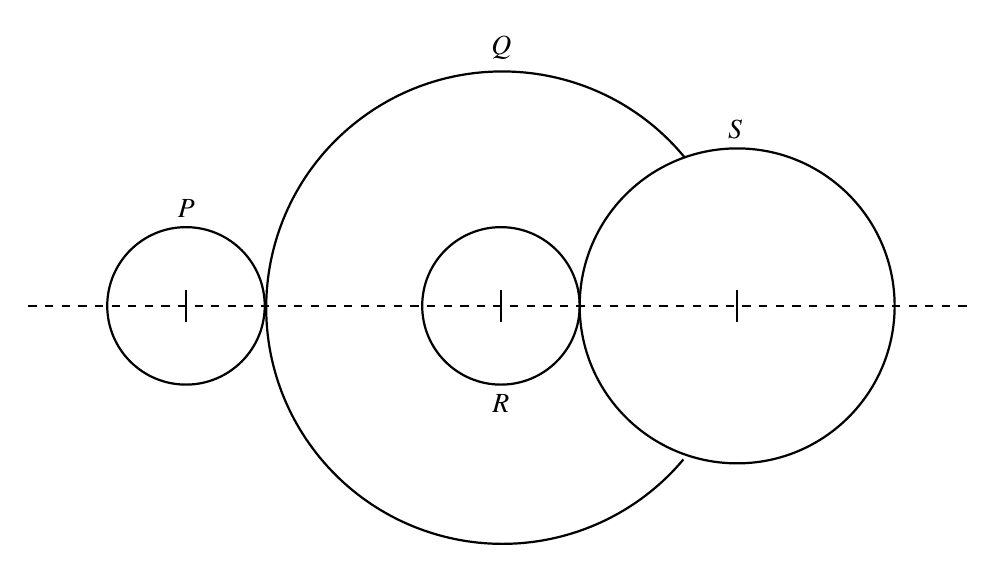
\begin{tikzpicture}
	\draw[draw=black, semithick, dashed] (-6,0) -- (6,0);
	\draw[draw=black, thick, solid] (-4,0) circle (1.00);
	\draw[draw=black, thick, solid] (2.333334,1.88563) arc[start angle=39.5, end angle=320, radius=3];
	\draw[draw=black, thick, solid] (0,0) circle (1.00);
	\draw[draw=black, thick, solid] (3,0) circle (2);
	
	\draw[draw=black, thick, solid] (-4,0.2) -- (-4,-0.2);
	\draw[draw=black, thick, solid] (0,0.2) -- (0,-0.2);
	\draw[draw=black, thick, solid] (3,0.2) -- (3,-0.2);
	
	\draw[] (-4,1) node[above] {$P$};
	\draw[] (0,-1) node[below] {$R$};
	\draw[] (0,3) node[above] {$Q$};
	\draw[] (3,2) node[above] {$S$};
\end{tikzpicture}
}
\end{center}
\hfill{\brak{\text{ME 2010}}}
\begin{enumerate}
\begin{multicols}{4}
\item $13.334$
\item $15.334$
\item $15.442$
\item $15.542$
\end{multicols}
\end{enumerate}

\item Annual demand for window frames is $10000$. Each frame cost $Rs.$ $200$ and ordering cost it $Rs.$ $300$ per order. Inventory holding cost is $Rs.$ $40$ per frame per year. The supplier is willing to offer $2\%$ discount if the order quantity is $1000$ or more, and $4\%$ if the order quantity is 2000 or more. If the total cost is to be minimized, the retailer should

\hfill{\brak{\text{ME 2010}}}
\begin{enumerate}
\begin{multicols}{2}
\item order 200 frames every time
\item accept $2\%$ discount
\item accept $4\%$ discount
\item order Economic Order Quantity
\end{multicols}
\end{enumerate}

\item The project activities, precedence, relationships and durations are described in the table. The critical path of the project is\\
\\\begin{table}[h!]    
  \centering
  \begin{tabular}{l >{\centering\arraybackslash}m{3cm} >{\centering\arraybackslash}m{3cm}}
    & \underline{Specific enthalpy \brak{kJ/kg}} & \underline{Velocity \brak{m/s}} \\[5pt]
    Inlet steam condition & $3250$ & $180$ \\
    Exit steam condition & $2360$ & $5$ \\
\end{tabular}


\end{table}\\

\hfill{\brak{\text{ME 2010}}}
\begin{enumerate}
\begin{multicols}{4}
\item P-R-T-V
\item Q-S-T-V
\item P-R-U-W
\item Q-S-U-w
\end{multicols}
\end{enumerate}
\end{enumerate}

\subsection*{Common Data Questions}
\begin{enumerate}

\item In a steam power plant operating on the Rankine cycle, steam enters the turbine at $4$ $MPa$, $350^\degree C$ and exits at a pressure of $15$ $kPa$. Then it enters the condenser and exits as saturated water. Next a pump feeds back the water to the boiler. The adiabatic efficiency of the turbine is $90\%$. The thermodynamic states of water and steam are given in the table.\\
\begin{table}[h!]    
  \centering
  \begin{tabular}{rl}
        Carbide tool: & $VT^{1.6}=3000$ \\
        HSS tool: & $VT^{0.6}=200$ \\
    \end{tabular}

\end{table}\\
$h$ is specific enthalpy, $s$ is specific entropy and $v$ is specific volume; subscripts $f$ and $g$ denote saturated liquid state and saturated vapour state.
\begin{enumerate}
\item The net work output \brak{kJ\text{ }kg^{-1}} of the cycle is
\hfill{\brak{\text{ME 2010}}}
\begin{enumerate}[label=(\alph*)]
\begin{multicols}{4}
\item $498$
\item $775$
\item $860$
\item $957$
\end{multicols}
\end{enumerate}

\item Heat supplied \brak{kJ\text{ }kg^{-1}} to the cycle is

\hfill{\brak{\text{ME 2010}}}
\begin{enumerate}[label=(\alph*)]
\begin{multicols}{4}
\item $2372$
\item $2576$
\item $2863$
\item $3092$
\end{multicols}
\end{enumerate}
\end{enumerate}

\item Four jobs are to be processed on a machine as per data listed in the table
\\\begin{table}[h!]    
  \centering
  \begin{tabular}[12pt]{ |c|c|c|}
    \hline
    \textbf{Job} & \textbf{Processing time \brak{\textbf{in days}}} & \textbf{Due Date } \\
    \hline
    $1$ & $4$ & $6$\\
    \hline 
    $2$ & $7$ & $9$\\
    \hline
    $3$ & $2$ & $19$\\
    \hline
    $4$ & $8$ & $17$\\
    \hline
\end{tabular}

\end{table}\\
\begin{enumerate}
\item If the Earliest DUe Date \brak{\text{EDD}} rule is used to sequence the jobs, the number of jobs delayed is

\hfill{\brak{\text{ME 2010}}}
\begin{enumerate}[label=(\alph*)]
\begin{multicols}{4}
\item $1$
\item $2$
\item $3$
\item $4$
\end{multicols}
\end{enumerate}

\item Using the Shortest Processing Time \brak{\text{SPT}} rule, total tardiness is

\hfill{\brak{\text{ME 2010}}}
\begin{enumerate}[label=(\alph*)]
\begin{multicols}{4}
\item $0$
\item $2$
\item $6$
\item $8$
\end{multicols}
\end{enumerate}
\end{enumerate}
\end{enumerate}

\subsection*{Linked Answer Questions}
\begin{enumerate}
\item A massless beam has a loading pattern as shown in the figure. The beam is of rectangular cross-section with a width of $30$ $mm$ and height of $100$ $mm$.
\\\begin{center}
   \scalebox{0.5}{\usetikzlibrary{patterns}
\begin{tikzpicture}

    \draw[thick] (0,0) node[above] {$A$} -- (16,0) node[above right] {$C$} ;
    \draw[thick] (8,2.5) -- (16,2.5);

    \draw[thick] (0,0) -- (-0.8,-1) -- (0.8,-1) -- (0,0);
    \draw[thick] (-0.8,-1) -- (-1.6,-1.8);
    \draw[thick] (0,-1) -- (-0.8,-1.8);
    \draw[thick] (0.8,-1) -- (0,-1.8);
    
    \draw[dashed] (0,0) -- (0,-5);
    \draw[dashed] (8,0) node[above left] {$B$} -- (8,-5);
    \draw[dashed] (16,0) -- (16,-5);
    
    \draw[thick] (16,0) -- (15.2,-0.6) -- (16.8,-0.6) -- (16,0);
    \draw[thick] (15.6,-0.8) circle (0.2);
    \draw[thick] (16.4,-0.8) circle (0.2);
    
    \draw[thick] (15.2,-1) -- (16.8,-1);
    \draw[thick] (15.2,-1) -- (14.4,-1.8);
    \draw[thick] (16,-1) -- (15.2,-1.8);
    \draw[thick] (16.8,-1) -- (16,-1.8);
    
    \draw[->] (4,-5) node[above, font=\Large] {$2000$} -- (0,-5);
    \draw[->] (4,-5) -- (8,-5);
    \draw[->] (12,-5) node[above, font=\Large] {$2000$} -- (16,-5);
    \draw[->] (12,-5) -- (8,-5);
    
    \draw[->] (8,2.5) -- (8,0);
    \draw[->] (9,2.5) -- (9,0);
    \draw[->] (10,2.5) -- (10,0);
    \draw[->] (11,2.5) -- (11,0);
    \draw[->] (12,2.5) node[above, font=\Large] {$3000$ $Nm^{-1}$}-- (12,0);
    \draw[->] (13,2.5) -- (13,0);
    \draw[->] (14,2.5) -- (14,0);
    \draw[->] (15,2.5) -- (15,0);
    \draw[->] (16,2.5) -- (16,0);

\end{tikzpicture}
}
\end{center}

\begin{enumerate}
\item The maximum bending moment occurs at

\hfill{\brak{\text{ME 2010}}}
\begin{enumerate}[label=(\alph*)]
\begin{multicols}{2}
\item Location B
\item $2675$ $mm$ to the right of $A$
\item $2500$ $mm$ to the right of $A$
\item $3225$ $mm$ to the right of $A$
\end{multicols}
\end{enumerate}

\item The maximum magnitude of bending stress \brak{\text{in }MPa} is given by

\hfill{\brak{\text{ME 2010}}}
\begin{enumerate}[label=(\alph*)]
\begin{multicols}{4}
\item $60.0$
\item $67.5$
\item $200.0$
\item $225.0$
\end{multicols}
\end{enumerate}
\end{enumerate}
\end{enumerate}
\end{document}

